\documentclass{article}

\usepackage{graphicx}
\usepackage[utf8]{inputenc}
\usepackage[T1]{fontenc}
\usepackage[francais]{babel}
\usepackage{hyperref}
\usepackage{amsmath,amsfonts,amssymb}
\usepackage{Tkz-Tab}
\usepackage{wrapfig}
\usepackage{verbatim}
\usepackage{array}

\begin{document}

\title{Gestion de flux dans le réseau
	\smallbreak
	TD n\degre4
	\smallbreak
	Modélisation mathématique
	\smallbreak
	Q4}
\author{Sibylle Roux \and Juliette Arazo \and Nicolas Le Gallo \and Tanguy Thomas}


\maketitle

\newpage

\tableofcontents

\newpage

\part{Etude statistique des temps interarrivés}

\section{Etude statistique des temps interarrivés pour tous les serveurs}

\subsection{Indicateurs de position et de dispersion}

\begin{center}
\begin{tabular}{cccc}
\hline
\hline
Min & Max & Moyenne & Médiane \\
\hline
0.01 & 21.98 & 2.9 & 1.95 \\
\hline
\hline
\end{tabular}
\end{center}

\begin{center}
\begin{tabular}{ccc}
\hline
\hline
Variance & Ecart-type & Etendue \\
\hline
8.73 & 2.95 & 22 \\
\hline
\hline
\end{tabular}
\end{center}

\begin{center}
\begin{tabular}{ccc}
\hline
\hline
Q1 & Q2 & Interquartile \\
\hline
0.76 & 4.09 & 3.33 \\
\hline
\hline
\end{tabular}
\end{center}

\subsection{Fonction de répartition}
\begin{center}
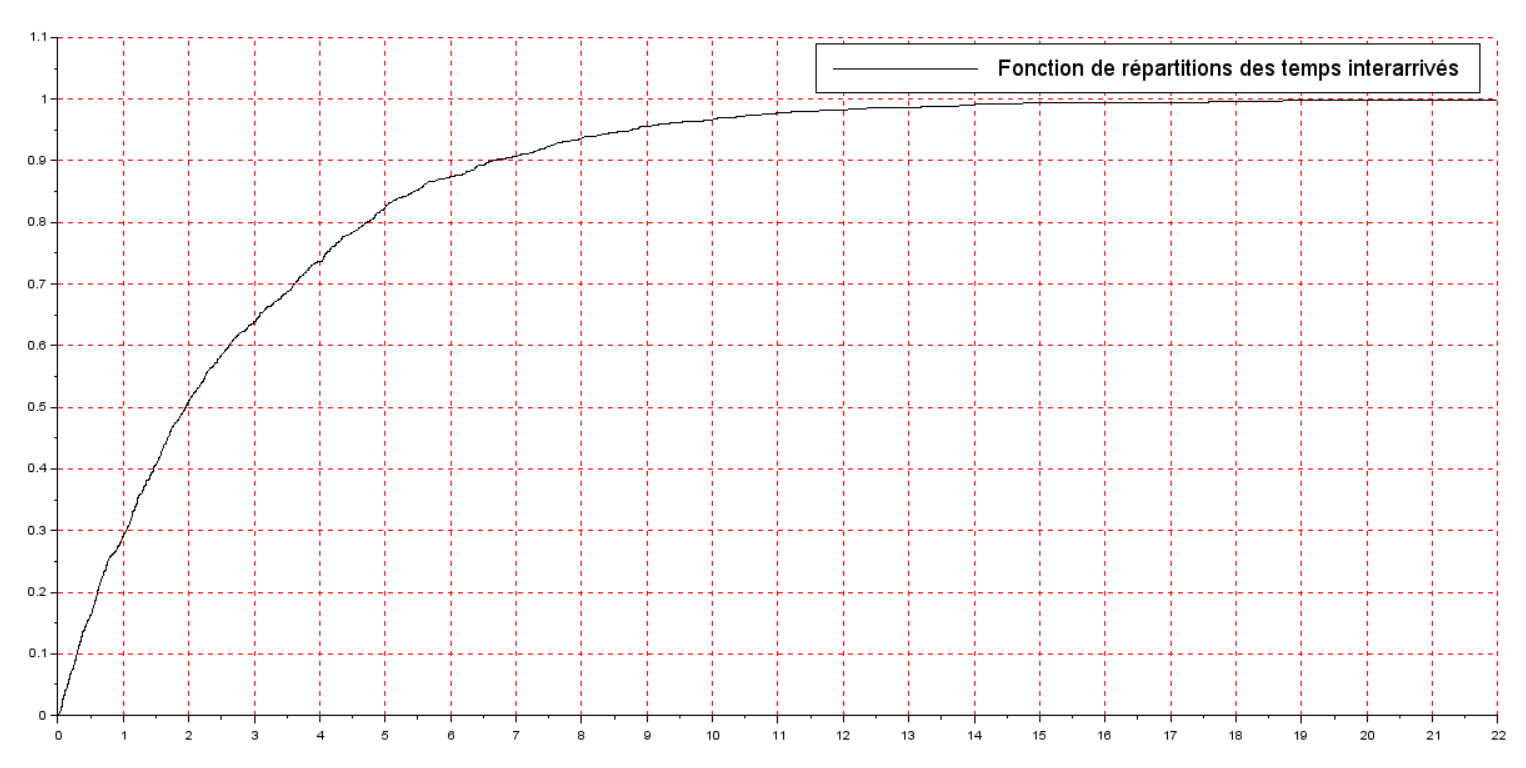
\includegraphics[width=450px]{img/repart.png}
\end{center}
\paragraph{}

\subsection{Histogramme}

\subsubsection{Histogramme avec classes isoamplitudes}
\begin{center}
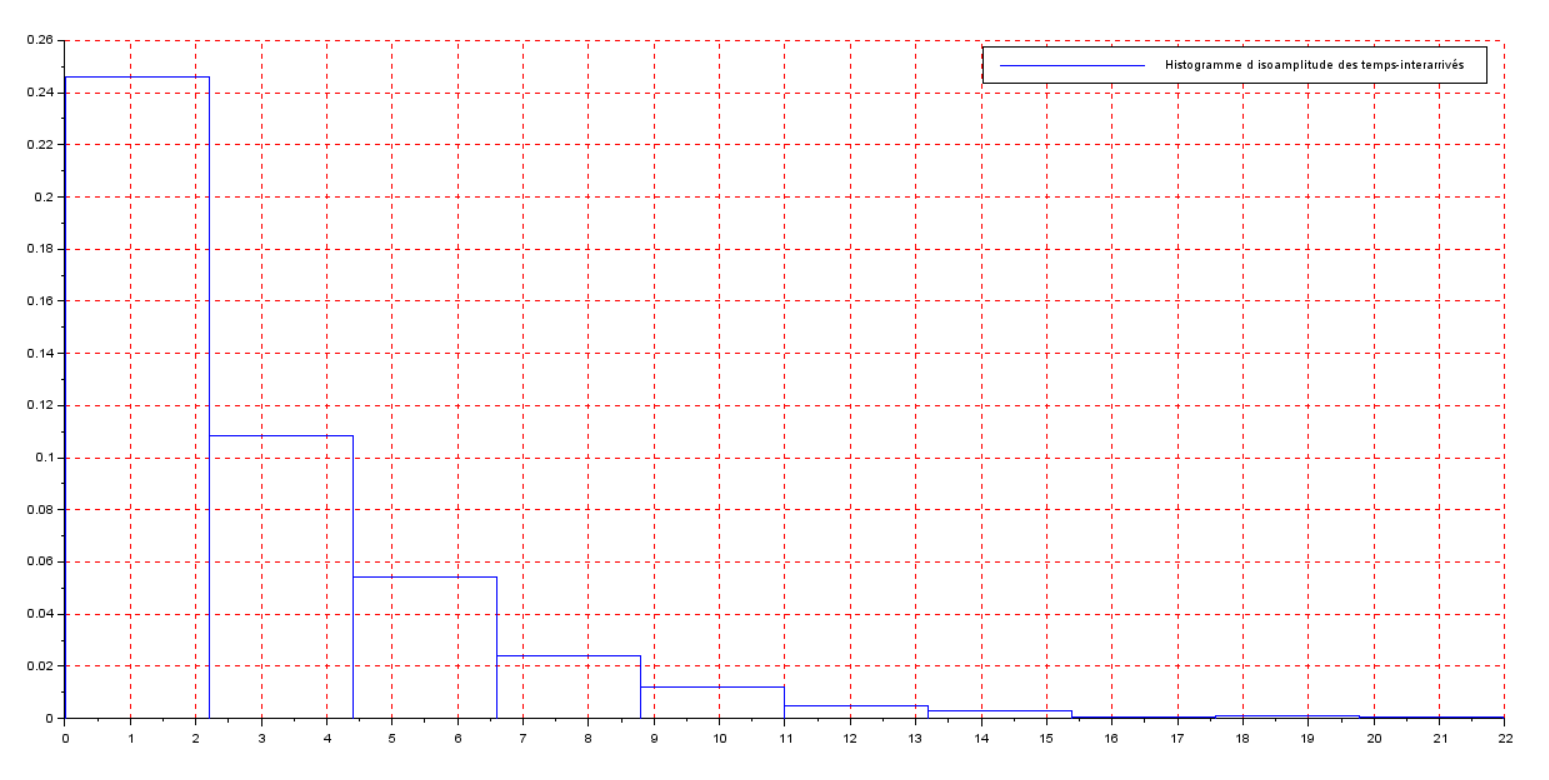
\includegraphics[width=450px]{img/H_isoa.png}
\end{center}
\paragraph{}

\subsubsection{Histogramme avec classes isofréquences}
\begin{center}
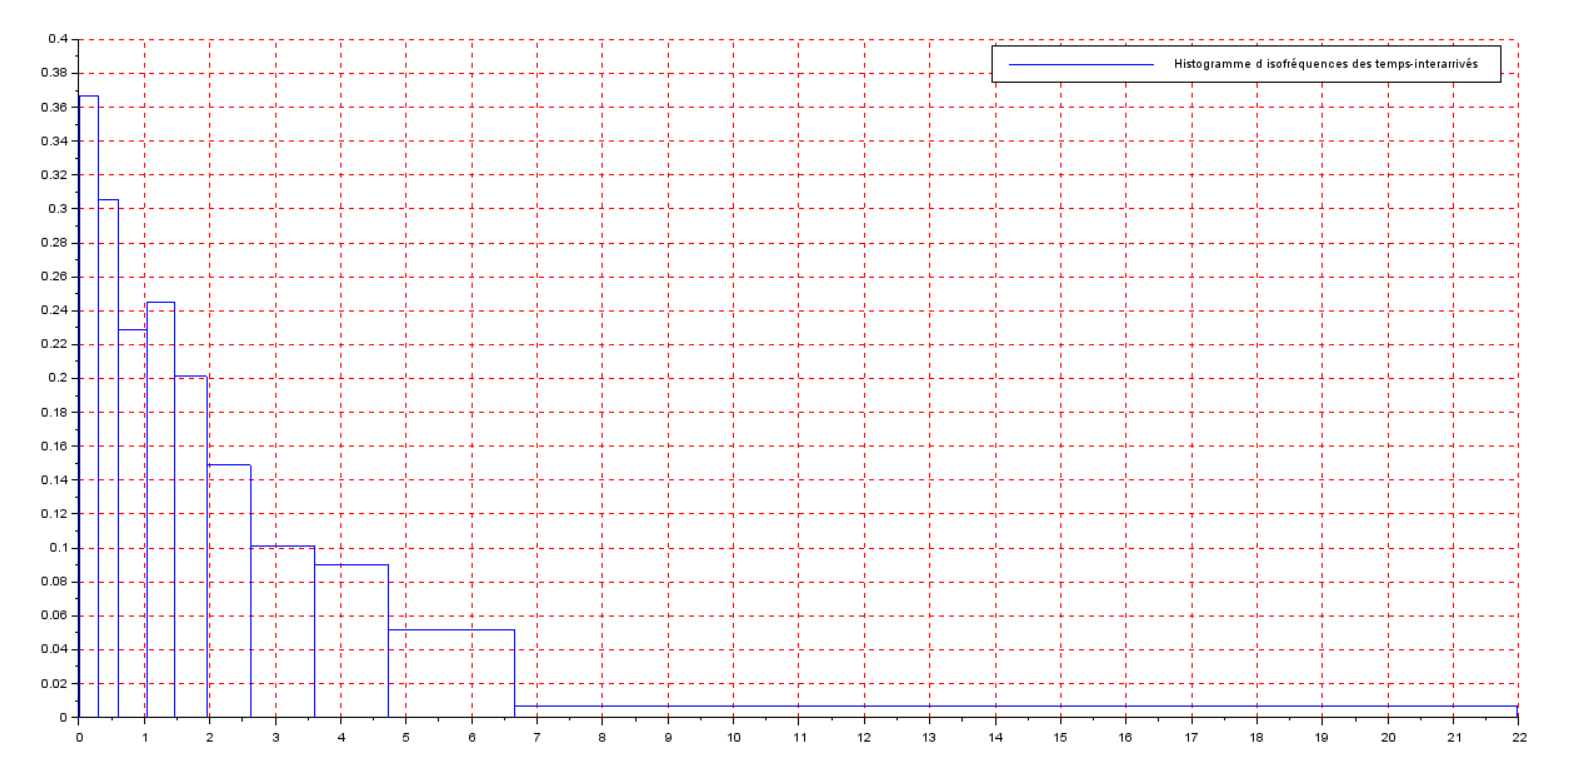
\includegraphics[width=450px]{img/H_isof.png}
\end{center}
\paragraph{}

\part{Etude statistique des temps de service}

\section{Indicateurs de position et de dispersion}

\begin{tabular}{|c|c|c|c|}
  \hline
  Indicateurs & Serveur 1 & Serveur 2 & Serveur 3 \\
  \hline
  Minimum & 0.01 & 0.04 & 0.01 \\
  Maximum & 134 & 88.9 & 68.6 \\
  Etendue & 134 & 88.8 & 68.6 \\
  Moyenne & 15.5 & 10.6 & 6.27 \\
  Médiane & 11.5 & 6.82 & 4.35 \\
  Q1 & 5.05 & 3.29 & 1.75 \\
  Q3 & 21.9 & 13.9 & 8.36 \\
  IQ & 16.8 & 10.6 & 6.61 \\
  Ecart-Type & 15 & 11.3 & 6.85 \\
  Variance & 225 & 127 & 46.9 \\
  \hline
\end{tabular}

\section{Fonctions de répartition}

\section{Histogrammes}

\paragraph{Histogramme}
\begin{center}
%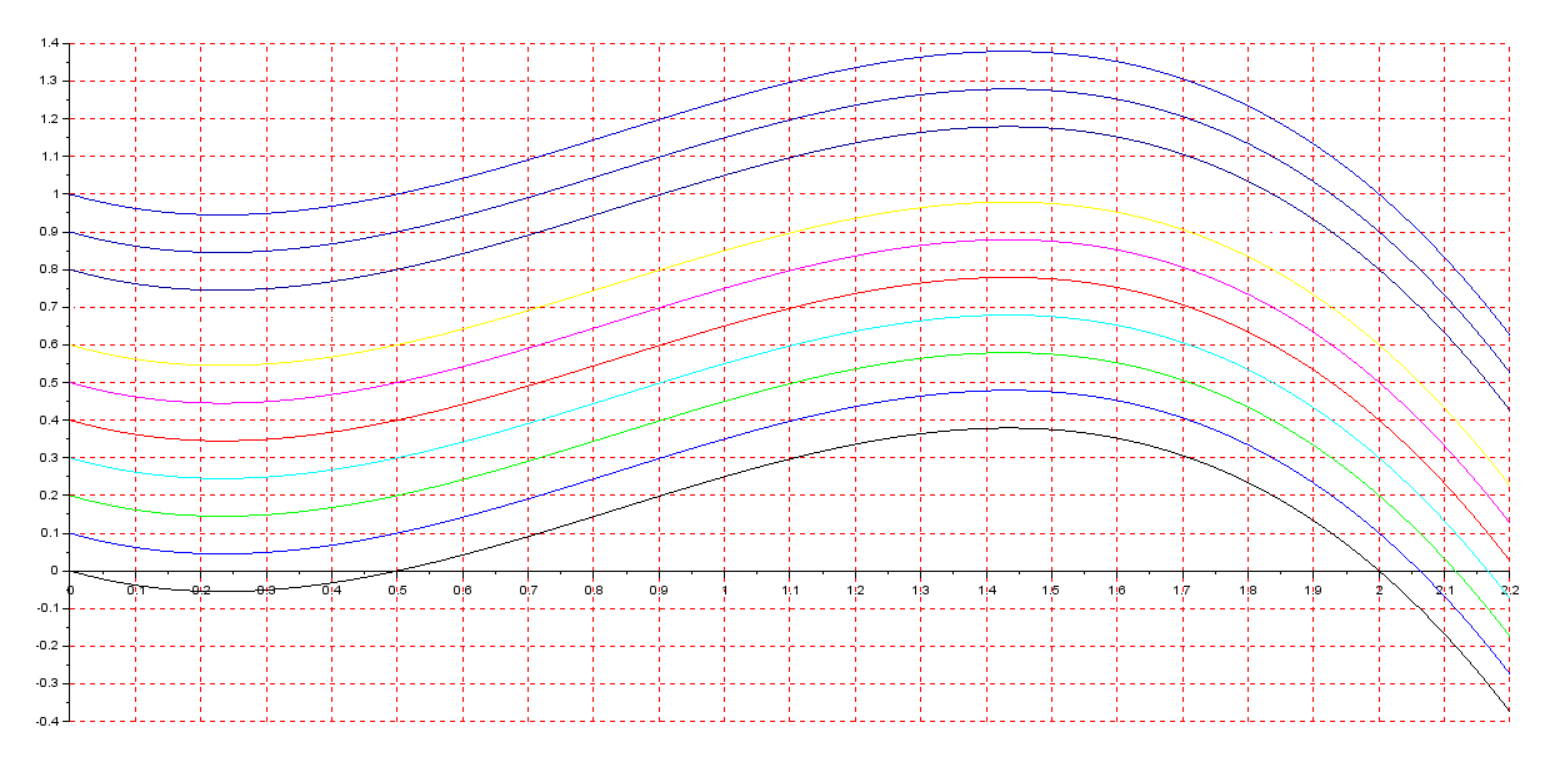
\includegraphics[width=300px]{img/part1/AlleeI.png}
\end{center}
\paragraph{}

\part{Ajustement graphique à des lois mathématique}

\section{Tous les serveurs}

\subsection{Ajustement à la loi uniforme}

\subsubsection{Estimation des paramètres}
\subsubsection{Superposition de la fonction de répartition}
\subsubsection{Superposition de la fonction de densité et de l'histogramme}

\subsection{Ajustement à la loi normale}

\subsubsection{Estimation des paramètres}
\subsubsection{Superposition de la fonction de répartition}
\subsubsection{Superposition de la fonction de densité et de l'histogramme}

\subsection {Ajustement à la loi exponentielle}

\subsubsection{Estimation des paramètres}
\subsubsection{Superposition de la fonction de répartition}
\subsubsection{Superposition de la fonction de densité et de l'histogramme}

\section{Serveur 1}

\subsection{Ajustement à la loi uniforme}

\subsubsection{Estimation des paramètres}
\subsubsection{Superposition de la fonction de répartition}
\subsubsection{Superposition de la fonction de densité et de l'histogramme}

\subsection{Ajustement à la loi normale}

\subsubsection{Estimation des paramètres}
\subsubsection{Superposition de la fonction de répartition}
\subsubsection{Superposition de la fonction de densité et de l'histogramme}

\subsection {Ajustement à la loi exponentielle}

\subsubsection{Estimation des paramètres}
\subsubsection{Superposition de la fonction de répartition}
\subsubsection{Superposition de la fonction de densité et de l'histogramme}

\section{Serveur 2}

\subsection{Ajustement à la loi uniforme}

\subsubsection{Estimation des paramètres}
\subsubsection{Superposition de la fonction de répartition}
\subsubsection{Superposition de la fonction de densité et de l'histogramme}

\subsection{Ajustement à la loi normale}

\subsubsection{Estimation des paramètres}
\subsubsection{Superposition de la fonction de répartition}
\subsubsection{Superposition de la fonction de densité et de l'histogramme}

\subsection {Ajustement à la loi exponentielle}

\subsubsection{Estimation des paramètres}
\subsubsection{Superposition de la fonction de répartition}
\subsubsection{Superposition de la fonction de densité et de l'histogramme}

\section{Serveur 3}

\subsection{Ajustement à la loi uniforme}

\subsubsection{Estimation des paramètres}
\subsubsection{Superposition de la fonction de répartition}
\subsubsection{Superposition de la fonction de densité et de l'histogramme}

\subsection{Ajustement à la loi normale}

\subsubsection{Estimation des paramètres}
\subsubsection{Superposition de la fonction de répartition}
\subsubsection{Superposition de la fonction de densité et de l'histogramme}

\subsection {Ajustement à la loi exponentielle}

\subsubsection{Estimation des paramètres}
\subsubsection{Superposition de la fonction de répartition}
\subsubsection{Superposition de la fonction de densité et de l'histogramme}

\newpage
\appendix

\section{Etude statistique des temps interarrivés}

\subsection{Indicateurs de position et de dispersion}
\begin{verbatim}
// Extraction des temps inter-arrivées
t_ia = data(2:$, 2) - data(1:1237, 2);

extremes = [min(t_ia), max(t_ia)] // calcul du min et du max
moyenne = mean(t_ia)  // calcul de la moyenne
mediane = perctl(t_ia,50) // calcul de la mediane

// calcul de la variance et de l'écart-type
v = variance(t_ia)
s = stdev(t_ia)

// calcul de l'étendue
etendue = extremes(2) - extremes(1)

Q1 = perctl(t_ia, 25) // premier quartile
Q3 = perctl(t_ia, 75) // troisième quartile
IQ = Q3(1) - Q1(1) // intervalle interquartile
\end{verbatim}

\subsection{Fonction de répartition}
\begin{verbatim}
// Extraction des temps inter-arrivées
t_ia = data(2:$, 2) - data(1:1237, 2);

tab = tabul(t_ia, 'i'); // construction du tableau des effectifs
tab(:,2) = tab(:,2)/length(t_ia); // calcul des fréquences
F = cumsum(tab(:,2)); // calcul des fréquences cumulées
plot2d2(tab(:,1),F)
legend("Fonction de répartitions des temps interarrivés")

// Définition des paramètres d'affichages
a=gca();
a.x_location = "origin";
a.grid=[5,5];

\end{verbatim}

\subsection{Histogramme}
\subsubsection{Histogramme avec classes isoamplitudes}
\begin{verbatim}
// Extraction des temps inter-arrivées
t_ia = data(2:$, 2) - data(1:1237, 2);

C = linspace(min(t_ia), max(t_ia), 11) // calcul des classes

histplot(C, t_ia, style=2) // dessine l'histogramme
legend("Histogramme d isoamplitude des temps-interarrivés")
\end{verbatim}
\subsubsection{Histogramme avec classes isofréquences}
\begin{verbatim}
// Extraction des temps inter-arrivées
t_ia = data(2:$, 2) - data(1:1237, 2);

deciles=perctl(t_ia,10:10:90) // Calcul des déciles
// Affectations d'isofréquences comme bornes de classes
for i=2:10
    ClassesDeciles(i)=deciles(i-1)
end
ClassesDeciles(1)=min(t_ia)
ClassesDeciles(11)=max(t_ia)

histplot(ClassesDeciles,t_ia,style=2) // dessine l'histogramme
legend("Histogramme d isofréquences des temps-interarrivés")
\end{verbatim}

\section{Etude statistique des temps de service}

\subsection{Indicateurs de position et de dispersion}

\subsubsection{Serveur 1}
\begin{verbatim}
// Extraction des temps de service
index_bool = ( data(:, 3) = 1 )
tabS1 = data(index_bool, :)
t_s1 = tabS1(1:$,4)

extremesS1 = [min(t_s1), max(t_s1)] // calcul du min et du max
moyenneS1 = mean(t_s1)  // calcul de la moyenne
medianeS1 = perctl(t_s1,50) // calcul de la mediane

// calcul de la variance et de l'écart-type
vS1 = variance(t_s1)
sS1 = stdev(t_s1)

// calcul de l'étendue
etendueS1 = extremesS1(2) - extremesS1(1)

Q1S1 = perctl(t_s1, 25) // premier quartile
Q3S1 = perctl(t_s1, 75) // troisième quartile
IQS1 = Q3S1(1) - Q1S1(1) // intervalle interquartile
\end{verbatim}

\subsubsection{Serveur 2}
\begin{verbatim}
// Extraction des temps de service
index_bool = ( data(:, 3) = 2 )
tabs2 = data(index_bool, :)
t_s2 = tabs2(1:$,4)

extremesS2 = [min(t_s2), max(t_s2)] // calcul du min et du max
moyenneS2 = mean(t_s2)  // calcul de la moyenne
medianeS2 = perctl(t_s2,50) // calcul de la mediane

// calcul de la variance et de l'écart-type
vS2 = variance(t_s2)
sS2 = stdev(t_s2)

// calcul de l'étendue
etendueS2 = extremesS2(2) - extremesS2(1)

Q1S2 = perctl(t_s2, 25) // premier quartile
Q3S2 = perctl(t_s2, 75) // troisième quartile
IQS2 = Q3S2(1) - Q1S2(1) // intervalle interquartile
\end{verbatim}

\subsubsection{Serveur 3}
\begin{verbatim}
// Extraction des temps de service
index_bool = ( data(:, 3) = 3 )
tabS3 = data(index_bool, :)
t_s3 = tabS3(1:$,4)

extremesS3 = [min(t_s3), max(t_s3)] // calcul du min et du max
moyenneS3 = mean(t_s3)  // calcul de la moyenne
medianeS3 = perctl(t_s3,50) // calcul de la mediane

// calcul de la variance et de l'écart-type
vS3 = variance(t_s3)
sS3 = stdev(t_s3)

// calcul de l'étendue
etendueS3 = extremesS3(2) - extremesS3(1)

Q1S3 = perctl(t_s3, 25) // premier quartile
Q3S3 = perctl(t_s3, 75) // troisième quartile
IQS3 = Q3S3(1) - Q1S3(1) // intervalle interquartile
\end{verbatim}

\begin{verbatim}
\end{verbatim}

\end{document}